\chapter{Background}\label{C:back}
Processing NMR relaxation in low SNR environments is crucial for dynamic environments such as well logging \cite{wellLoggingBook} \cite{UsingNMRPetrophysicalKenyon1992nuclear}. The previously published work forms the benchmark for comparison with this project's proposed technique. This background survey details the current published technique, the evaluation criteria of the techniques, and the Bayesian theory that informs the design in Chapter \ref{C:design}.

\section{NMR Relaxation}
Nuclear magnetic resonance involves determining the nature of the nuclei of a sample by using its magnetic behaviour \cite{NMRSignalProcessingBook}. To provide an effective basis for the signal processing techniques to operate on, we start by examining the physics of the magnetism of the nuclei.



\subsection{Underlying Physics}

\subsubsection{Magnetism of the Nuclei}
The nucleus has two classical aspects that make it a microscopic magnet \cite{NMRSignalProcessingBook}:
\begin{enumerate}
    \item a nucleus has an electrical charge from the protons that make it up, and
    \item it may have a non-zero spin.
\end{enumerate}
The spin creates a magnetic dipole moment, $\vec{\mu}$. This phenomenon is expressed as the relation of angular momentum $\vec{J}$ and the gyro-magnetic ratio inherent to the nuclei, $\gamma$, such that

\begin{equation}
    \vec{\mu} = \gamma \vec{J}
    \label{eq:magneticMomentEquation}
\end{equation}
A macroscopic magnetic field formed by many nuclei, $\vec{M}$, is the summation over the total number of spins in the system, $N_s$  \cite{NMRSignalProcessingBook}.

\begin{equation}
    \vec{M} = \sum^{N_s}_{n = 1}\vec{\mu_{n}}
    \label{eq:macroMagnetic}
\end{equation}

Introducing a static magnetic field $B_0$ induces rotation of the magnetic moments of the nuclei. This rotation about the axis of $B_0$ is called nuclear precession. The angular frequency of this rotation is known as the Larmor frequency  \cite{NMRSignalProcessingBook}. This is given by: 
\begin{equation}
    \omega_0 = \gamma B_0
    \label{ref:LarmorFreq}
\end{equation}
Holding the magnetic field $B_0$ constant means that all the same nuclei exhibit nuclear precession at the same frequency. Their magnetic dipoles precess at the same frequency.

In order to set all of the rotations of magnetic dipoles into the same phase we require another magnetic field, $B_1$. This field makes the system phase coherent  \cite{NMRSignalProcessingBook}. This is so that all of the magnetic dipoles of the same frequency constructively interfere, providing a strong enough signal to measure. $B_1$ is in the form of a short RF (radio frequency) pulse that lasts from microseconds to the milliseconds  \cite{NMRSignalProcessingBook}.

With phase coherence achieved there is a measurable macroscopic magnetic field originating from the nuclei. The change of this nuclei magnetic field is described by the Bloch Equation  \cite{NMRSignalProcessingBook}:
\begin{equation}
    \frac{d\vec{M}}{dt} = \gamma \vec{M} \times \vec{B} - \frac{M_{x}\vec{i} + M_{y}\vec{j}}{T_2} - \frac{(M_z - M_{z}^0)\vec{k}}{T_1}
    \label{eq:blochEquation}
\end{equation}
where $\vec{M} = (M_x, M_y, M_z)$.
\subsubsection{Relaxation}

At the end of an RF pulse, the magnetic field $B_1$ is set to 0  \cite{NMRSignalProcessingBook}. In the rotating frame of reference this eliminates the first term of the Bloch equation. This results in the magnetism of the system of nuclei to be described by two differential equations:
\begin{equation}
    \begin{cases}
          \frac{dM_{z'}}{dt}    =         -\frac{M_{z'} - M_{z}^0}{T_1}  \\
           \frac{dM_{x'y'}}{dt}    =         -\frac{M_{x'y'}}{T_2}  \\         
    \end{cases}
\end{equation}
The time evolution of the system is governed by these equations. Immediately after the RF pulse ($t = 0_+$) for the transverse magnetic field, $M_{x'y'}$, is expressed as:

\begin{equation}
    M_{x'y'}(t) = M_{x'y'}(0_+) e^{-t/T_2}
    \label{eq:T2ExpoenetialRelaxation}
\end{equation}

This exponential decay is referred to as the $T_2$ relaxation  \cite{NMRSignalProcessingBook}. The decay constant $T_2$ is used to give insight to the physical properties of the nuclei in the sample. This exponential model is only suitable for weak spin-spin systems such as fluids. Therefore, the analysis of the $T_2$ relaxation is limited to the behaviour of the fluids in a sample.

\subsubsection{Detecting Relaxation}
The resultant magnetic field can be detected by using Faraday's Law and the principle of reciprocity \cite{NMRSignalProcessingBook}:

\begin{equation}
    V(t) = -\frac{\partial \Phi(t)}{\partial t} = - \frac{\partial}{\partial t} \int_\text{object} \vec{B_r}(\bm{r}) \cdot \vec{M}(\bm{r} \cdot t) d \bm{r}
    \label{eq:detectionFaraday}
\end{equation}

$\vec{B_r}(\bm{r})$ is the magnetic field produced by the coil by a hypothetical unit direct current. After demodulation of the voltage \cite{NMRSignalProcessingBook}, we get a measurement signal we can process and analyse:

\begin{equation}
    m(t) = \int_{\text{object}} M_{x,y}(\bm{r}, 0 )e^{i\gamma \Delta B(\bm{r})t} d \bm{r}
    \label{eq:detectionFinalSignal}
\end{equation}
The term $\Delta B $ varies in space due to the inhomogeneity of the magnetic field. This is a form of error introduced into the measurement process, which is more pronounced in field measurement tools rather than in laboratory tools. Figure \ref{fig:example_field_tool} illustrates an example field measurement tool and its grossly inhomogeneous magnetic field.

\begin{figure}[htb]
    \centering
    \includegraphics[width=0.75\textwidth]{backgroundImages/example_of_tool}
    \caption{An example of a field measurement tool used to detect relaxation for the rock in a bore hole \cite{nmr_picture_tool}}.
    \label{fig:example_field_tool}
\end{figure}



\subsection{The $T_2$ Density Function}
The density function of T2 relaxation times is denoted by $f(T_2)$. An example $T_2$ distribution is shown in Figure \ref{fig:theModel}. The T2 density function forms the basis of analysis of fluids in a sample. There are several properties that relate T2 relaxation to fluids in porous media. The most significant two we shall analyse are: \textit{porosity}, and \textit{bound fluid fraction} \cite{NMRForRockskleinberg1993nuclear} \cite{wellLoggingBook}.

\begin{figure} [h]
    \centering
    \begin{subfigure}[b]{0.495\textwidth}
        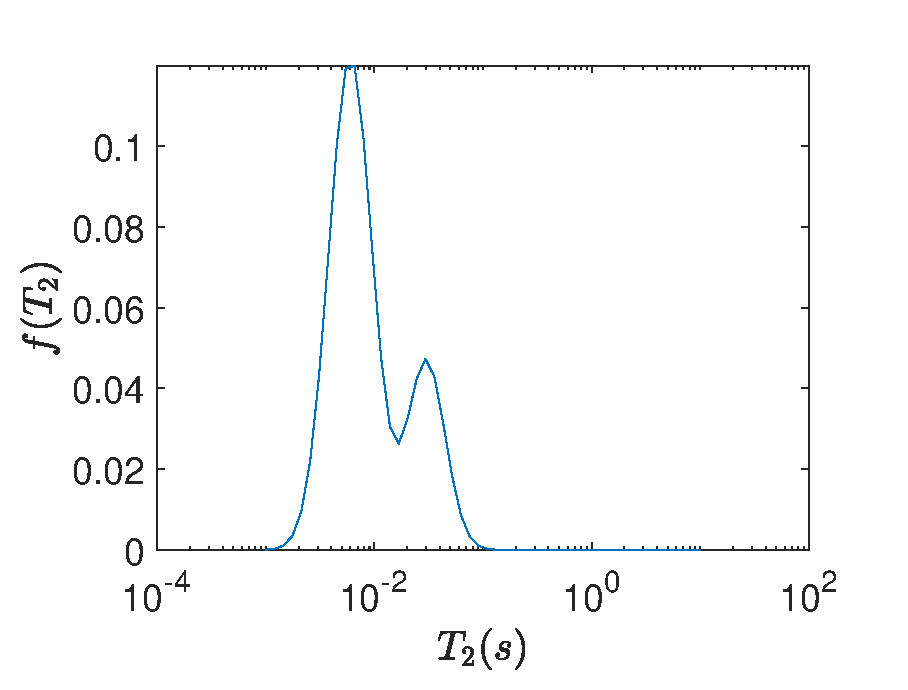
\includegraphics[width=\textwidth]{backgroundVector/densityFunction.eps}
        \subcaption{The density function $f(T_2)$}
        \label{fig:densityFunction}
    \end{subfigure}
    \begin{subfigure}[b]{0.495\textwidth}
        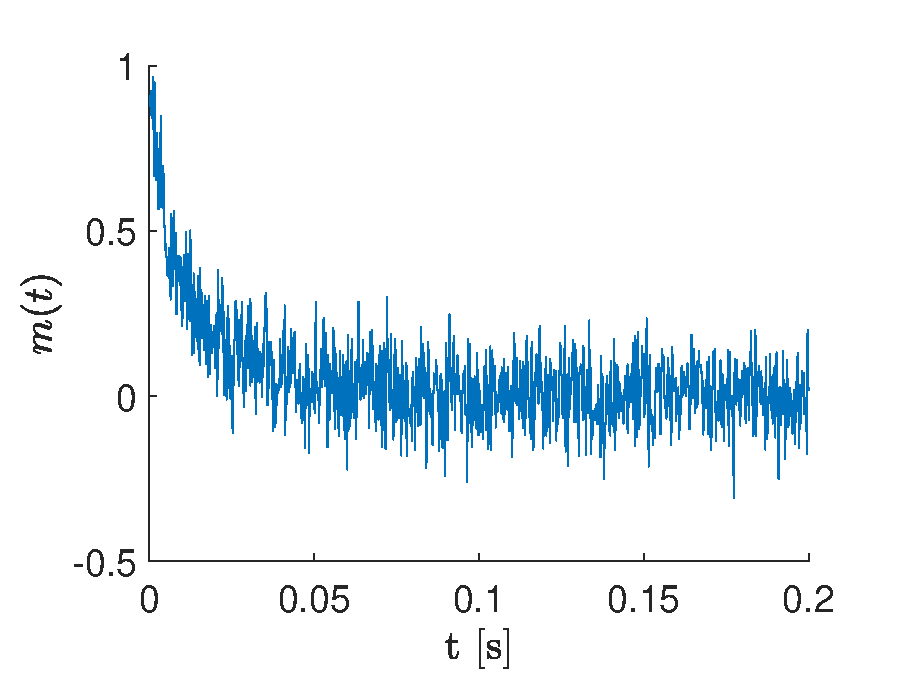
\includegraphics[width=\textwidth]{backgroundVector/measured.eps}
        \subcaption{The modelled measured data $m(t)$}
        \label{fig:measuredData}
    \end{subfigure}
    
    \caption{An example modelled $T_2$ density function and the measured data generated from it. It has unity porosity and a noise standard deviation of $\sigma_\epsilon = 0.2$}
    \label{fig:theModel}
\end{figure}

\subsubsection{Porosity}
The fraction of the rock volume that can be occupied by fluid is defined as the porosity ($\phi$) \cite{PorosityandT2Times}. After calibration with a water sample ($\phi = 1$), the integral over the entire density function is equal to the porosity.
\begin{equation}
    \label{eq:porosity_defn}
    \phi = \int_0^\infty f(T_{2}) dT_{2}
\end{equation}
This is approximated by taking the sum over the discretised density function:
\begin{equation}
    \phi \approx \sum_i f(T_{2 i})
\end{equation}

\subsubsection{Bound Fluid Fraction}
Bound fluids are fluids that require significant capillary pressure to remove from porous media \cite{wellLoggingBook}. This pressure is caused by the fluid being located in small pores of the media. The volume of bound fluids -- the bound fluid volume (BFV) \footnote{also known as the bulk fluid irreducible (BVI)} -- is associated with relaxation times below a cut off value, $T_{c}$ \cite{wellLoggingBook}. This volume is obtained with:
\begin{equation}
    BFV = \int^{T_{c}}_{0} f(T_2) d T_2
    \label{eq:boundFluidVolume}
\end{equation}
Free fluids conversely are fluids that are able to be extracted since they experience less capillary pressure restraining them \cite{NMRForRockskleinberg1993nuclear}\cite{BoundfluidFractionchen1998improving}. Therefore, the free fluid volume -- also known as movable fluids (BVM) -- can be expressed as the remaining fluid that is not bound, having its T2 relaxation above the cut-off. Since the porosity is defined to be all of the fluid volume in the sample, the bound fluid fraction (BFF) can be expressed in terms of the porosity. 

The bound fluid fraction is expressed, as:
\begin{equation}
    BFF = 
    \frac{BFV}{BFV + BVM} =
    \frac{BFV}{\phi} = \frac{\int^{T_{c}}_{0} f(T_2) d T_2}{\int_0^\infty f(T_{2}) dT_{2}}
    \label{eq:boundFluidFraction}
\end{equation}




\section{Inversion of Measured Data}
In order to compute the T2 relaxation times from the measured data we require a computational model that corroborates with the physical model. This model reveals that the measured data is ill-posed for an inversion problem.

\subsection{Model of T2 Relaxation Measurements} \label{subsec:modelT2relaxation}
The measured T2 relaxation of a sample can be modelled with the following integral
\begin{equation}
    m(t) = \int e^{\frac{-t}{T_2}} f(T_2) dT_2 + \epsilon
    \label{eq:T2RelaxationModelContinuous}
\end{equation}
As we are unable to numerically compute continuous functions, we discretise this into
\begin{equation}
    \hat{m}(t) = \sum^{N_y}_{k = 1} f_k e^{\frac{-t}{T_{2_k}}} + \epsilon
    \label{eq:T2RelaxationModel}
\end{equation}
This model corresponds with the detected exponential decay of the transverse magnetic field in (\ref{eq:T2ExpoenetialRelaxation}). The measurement data $m$ is made up of $N_2$ discrete measurements. The time constants of these exponential functions -- $T_{2_k}$ -- make up the T2 relaxation times. In the model itself $N_y$ is the total number of relaxation times modelled, $f_k$ is the contribution of each exponential, and $\epsilon$ is the additive white Gaussian noise introduced by the measurement process.

Since we know the measurements are made of exponentially decaying functions, we can construct an exponential kernel matrix, $K$, that maps from the T2 domain to the time domain, i.e.

\begin{equation}
    (K)_{ij} = e^{-t_i / T_{2,j}}
\end{equation}

Hence, the T2 density function is modelled as a vector $f$. The overall model of the measurement process is described as:
\begin{equation}
    m = Kf + \epsilon \text{, where } m \in \mathbb{R}^{N_2} \text{, } f \in \mathbb{R}^{N_y} \text{, } K \in \mathbb{R}^{N_2 \times N_y} \text{, } \epsilon \in \mathbb{R}^{N_2}
    \label{eq:T2RelaxationModelMatrices}
\end{equation}



\subsection{Ill-posed Nature}
The goal of this project is to find the bound fluid fraction. This has traditionally required estimating $f$ and then computing from there with an integral via (\ref{eq:boundFluidFraction}). Transforming a \textit{noiseless} single exponential to an easily quantifiable time constant can be achieved with the Inverse Laplace Transform (ILT) \cite{BulterReedsDawsonMethod1981}.
\begin{equation}
   f_k\delta   \bigg(   \frac{1}{T_{2}} - \frac{1}{T_{2_k}} \bigg) = \mathcal{L}^{-1} \bigg\{ f_k e^{\frac{-t}{T_{2_k}}} \bigg\}
    \label{eq:InverseLaplaceNaive}
\end{equation}
However, this non-robust version of the ILT is not suited for the noisy model. There can be very different results for the same measured sample due to the random effect of noise. Also, the kernel matrix $K$ is very poorly conditioned for computation \cite{NumericalFredholm1971hanson1971numerical}. The measured signal cannot be frequency filtered since that process does not discriminate between the noise or the true signal. This necessitates the implementation of a robust numerical approximation of the inversion of measurement data.





\section{Existing Techniques}
\label{Sec:existing_techniques}
The typical design limitation of the existing techniques is their limit on prior information for the sake of generality. The main thrust of these previous designs to add more ways of evaluating error without relaxing the constraint on useful prior information. The preferred form of deriving the density function is also via an iterative computation rather than a direct analytic approach.


\subsection{Technique Constraints}\label{subsection:techniqueConstraints}

The existing techniques have constraints that limit their accuracy in estimation in exchange for generality. These include:
\begin{itemize}
    \item knowing only the measurement, $m$, and the noise power of it, $\sigma$, 
    \item that the density function $f$ is non-negative,
    \item that the measurement is in the form of a decaying exponential, and
    \item the sample period of the measurements is known.
\end{itemize}
These constraints imply that more detailed prior information may allow for a greater reduction in error in comparison to the existing techniques. This potential performance increase is fundamental for the design of the Bayesian estimator in Chapter \ref{C:design}.




\subsection{The Inverse Laplace Transform (ILT) Technique} \label{section:ILT}

Numerical inversion is based on the goal of minimising the difference between the true unknown distribution and the estimated distribution. The most popular inversion technique of T2 relaxation is that described by Venkataramanan et al.. for one dimensional and two dimensional distributions \cite{Venk2DFredholm2002} \footnote{The ILT technique explored here is technically solving Fredholm integrals of the first kind.}. This technique requires knowing the standard deviation of the noise present, $\sigma_\epsilon$.

\subsubsection{Inversion With Optimisation}
The Bulter-Reeds-Dawson (BRD) method \cite{BulterReedsDawsonMethod1981} provides the established technique for robust numerical computation of the ILT. This is an optimisation framework expressed as:
    
\begin{equation}
    \Phi(f) = \min_{f\geq0}  ||Kf_\alpha - m||^2 + \alpha||f_{\alpha}||^2
    \label{eq:minimseError1981Optimise}
\end{equation}    
In this framework we can see that the main cost being minimised is the difference between the hypothesised noiseless time domain data $Kf_\alpha$ and the actual measured data $m$. However, constricting the problem simply to just this allows for overfitting to the noise itself. To counteract this, the second term $\alpha||f_{\alpha}||^2$ is added to penalise the size of the hypothesised density function. This `smooths' the hypothesised $f$ to prevent it fitting to the noise \cite{RegularizationElden1977algorithms}. This process is known as \textit{regularisation}.
The BRD method \cite{BulterReedsDawsonMethod1981} sets the optimal regularisation parameter as
\begin{equation}
    \alpha_{\text{opt}} =  \frac{N_y \sqrt{ \sigma_{\epsilon} } }{||c||} 
    \text{, }
    \label{eq:optAlphaOptimise}
\end{equation} 
where the vector $c$ satisfies the following simultaneous equations \cite{BulterReedsDawsonMethod1981}:
\begin{equation}
    f_{\text{est}} = \text{max}(0, Kc)
    \label{eq:optC1}
\end{equation}  
\begin{equation}
    (Kf - g) + \alpha c = 0
    \label{eq:optC2}
\end{equation}  
    This method involves updating $c$ with $\alpha_{\text{opt}}$ and then computing $\alpha_{\text{opt}}$ for the new $c$ (Figure \ref{fig:2002Optimisation}). This iterative computation converges towards the density function we are trying to predict after approximately 20 iterations. The problem is convex \cite{BulterReedsDawsonMethod1981}, so the starting $\alpha$ and $c$ can be set to any value as it will automatically converge to the optimal solution. 

\begin{figure}[ht!]
    \centering
    \includegraphics[width=\textwidth]{backgroundVector/BlockDiagram2002Optimisation.pdf}
    \caption{Computational work flow of the optimisation framework in the inverse Laplace transform approximation}
    \label{fig:2002Optimisation}
\end{figure}

\subsubsection{Calculating $c$}
    Computing the $c$ vector can be computationally dangerous due to potential error introduced by the inversion of a possibly ill behaved matrix \cite{BulterReedsDawsonMethod1981}. The BRD method circumvents this problem by ensuring inversion is done by a positive semidefinite matrix: 
 
\begin{equation}
    H = \text{step}(KK^T) \text{  , where} \quad \text{step}(t) = 
    \begin{cases}
    1  & t \geq 0\\
    0  & t < 0
    \end{cases}
    \label{eq:makeSemiPostiveDefinite}
\end{equation}   
that feeds in the regularisation coefficient \cite{BulterReedsDawsonMethod1981} $\alpha$ to give
\begin{equation}
    c =  (KHK^T + \alpha I)^{-1} m \text{.} 
    \label{eq:optFindC}
\end{equation} 


\subsubsection{Measurement Data Compression} \label{section:compression}
To reduce computation time, truncated singular value decomposition of the kernel is used \cite{Venk2DFredholm2002}. Starting with the singular value decomposition $K = U S V^T$:
\begin{itemize}
    \item the first $n$ columns $\hat{U}$ and $\hat{V}$ are kept from $U$ and $V$, and
    \item the first $n$ columns and rows of $\hat{S}$ are kept from S \cite{TSVDHansen1987truncatedsvd}.
\end{itemize}

\begin{equation}
    \hat{K} = \hat{S} \hat{V}^T
    \label{eq:compressedKernel}
\end{equation}
\begin{equation}
    \hat{m} = m^T \hat{U}
    \label{eq:compressedMeasurement}    
\end{equation}

These are then used to make a new kernel and measurement vector. Here, the dimensionality is reduced from $N_2$ (thousands) dimensions to $n$ dimensions. The optimisation problem remains unchanged as $||K||^2 = ||USV^T||^2 \approx ||SV^T||^2$; we are typically minimising the same error. This holds because the singular values of $K$ decay very rapidly as it is an exponential kernel \cite{NumericalInversionLaplaceTransform1978}.



\subsection{Direct Tapered Area Estimation Technique} \label{ss:taperedAreas}
Tapered areas are weighted areas under a T2 distribution \cite{TaperedAreaskleinberg1997tapered}. This is a property of the density function that corresponds to bound fluid volume and porosity. Therefore, it is a viable candidate for estimating the bound fluid fraction of a sample directly from measurement data \cite{GruberLinearFunctionals2013}.

Tapered areas are computed directly from a density function with the use of a tapered step function. The specific transform used by Gruber et al. is the Exponential Haar Transform (EHT) \cite{GruberLinearFunctionals2013}. This is defined in the $T_2$ domain as:

\begin{equation}
    K_a(T_2, T_c) = \frac{C}{\gamma}\tanh(\alpha \gamma) 
    \label{eq:expHaarTransformT2}
\end{equation}
In addition, the EHT is defined in the time domain as:
\begin{equation}
    k_a(t, T_c) = C(-1)^n e^{\beta t} \text{, } \quad 2n\alpha < t < 2(n+1)\alpha \text{,}   \quad n \in \mathbb{Z}
    \label{eq:expHaarTransformTime}
\end{equation}
The actual tapered area ($B$) and the estimate tapered area ($\hat{B}$) are computed with an inner product \footnote{This is equivalent to an integral transform for the continuous case.} of the EHT kernel and the data for their respective domains:

\begin{equation}
   \label{eq:estTaperedAreas}
   B = K_a(T_2,T_c)f(T_2),  \quad \hat{B} = k_a(t, T_c)m(t)
\end{equation}
The transform in the $T_2$ domain is normalised so that where $T_2 = T_c$, $K = 0.5$ \cite{GruberLinearFunctionals2013}. To meet this property, the constants are set by Gruber et al. to be:
\begin{equation}
    C = \frac{0.7213}{T_c} \text{, } \quad \alpha = (1.572)T_c \text{, } \quad
   \beta = \frac{0.4087}{T_c}  \text{, } \quad \gamma = \frac{1}{T_2} + \beta  
   \label{eq:haarTransformConstants}
\end{equation}









\subsection{The ILT+ Technique}
More recent techniques have refined the optimisation approach with additional measures of evaluating estimation error. These come in the form of more prior information used to compensate for the high noise environment of the measured data \cite{GruberT2Estimation2013}. This involves calculating aspects that are intrinsic to the T2 density function. These are known as linear functionals. The two main functionals used for this improved optimisation framework are \textit{moments} and \textit{tapered areas} (Figure \ref{fig:2013ILTXOptimisation}) \cite{GruberT2Estimation2013}.


\begin{figure}[ht!]
    \centering
    \includegraphics[width=\textwidth]{2013_ILT+.pdf}
    \caption{Computational work flow of the optimisation framework for the ILT+ method.}
    \label{fig:2013ILTXOptimisation}
\end{figure}

\subsubsection{Estimation of Moments} \label{section:moment_estimation}
A moment is a description of the `weight' of the density function on the T2 axis \cite{VenkMellin2010}. An example of a moment is the first moment, the mean. The $\omega^{\text{th}}$ moment is defined as:

\begin{equation}
    \langle T_2^{\omega}  \rangle \equiv
    \frac
    {\int_{0}^{\infty}  T_2^{\omega} f_{T_2}(T_2)dT_2}
    {\int_{0}^{\infty}  f_{T_2}(T_2)dT_2 }
    =     
    \frac
    {\int_{0}^{\infty}  T_2^{\omega} f_{T_2}(T_2)dT_2}
    {\phi}
    \label{eq:defnMoment}
\end{equation}
The ILT+ requires an estimation of the moment directly from the measured data without knowledge of the density function. This estimation is implemented using the Mellin transform (MT) \cite{VenkMellin2010}:

\begin{equation}
\langle \hat{T_2^{\omega}}  \rangle =
\begin{cases}
        \frac{-1}{\Gamma (\mu) \phi}
        \int_{0}^{\infty}t^{\omega -1}[m(t) - \phi]dt &
        \text{ $-1<\omega<0$,}\\
        1 & \text{ $\omega=0$,}\\
        \frac{1}{\Gamma (\mu) \phi}
        \int_{0}^{\infty}t^{\omega -1}m(t)dt &
        \text{ $\omega>0$,}\\
\end{cases}
\label{eq:mellinTransform}
\end{equation}

The computed moment is a numerical value describing the density function. This has a propagated uncertainty described in \cite{VenkMellin2010} that can be used to evaluate how much we should depend on it for the optimisation framework.


\subsubsection{Estimation of Tapered Areas}
This linear functional is discussed in Section \ref{ss:taperedAreas}. The implementation is identical with the only difference being that the result is fed into the ILT+ framework.


\subsubsection{Constrained Optimisation}
    Directly estimated linear functionals are introduced as additional methods of evaluating the estimate density functions' error \cite{GruberT2Estimation2013}. These estimated functionals are also more accurate than simply using the ILT method \cite{GruberLinearFunctionals2013}. Therefore, the additional prior information yields a more accurate estimation of the density function in a low SNR environment. This forms the basis for the ILT+ method \cite{GruberT2Estimation2013}. The optimisation framework that aims to minimise the cost $Q(f_\alpha)$ takes the form of:
\begin{equation}
    Q(f_\alpha) = \min_{f\geq0}  ||W(Lf_\alpha - g)||^2 + \alpha||f_\alpha||^2
    \label{eq:2013Optimise}    
\end{equation}
    This framework is adapted from the ILT method (eq. \ref{eq:minimseError1981Optimise}) by appending the estimations and uncertainties of the tapered areas and moments onto the framework \cite{GruberT2Estimation2013} such that:
 \begin{equation}
    g = 
    \begin{bmatrix}
    \hat{m}  \\
    \langle T_2^{\omega_1} \rangle \\
    \vdots \\
    \langle T_2^{\omega_{N_{m}}} \rangle \\
    B_1 \\
    \vdots \\
    B_{N_{a}}
    \end{bmatrix}
    \text{, } \quad
    L = 
    \begin{bmatrix}
    \hat{K}  \\
    \frac{1}{\phi}T_{2}^{\omega_1}\\
    \vdots \\
    \frac{1}{\phi}T_{2}^{\omega_{N_{m}}}\\    
    K_{a}(T_2,T_{c_{1}}) \\
    \vdots \\
    K_{a}(T_2,T_{c_{3}})     
    \end{bmatrix}
    \text{, } \quad
    W = 
    \begin{bmatrix}
    \frac{1}{\sigma_\epsilon}  \\
    \frac{1}{\sigma_{\omega_1}}  \\ 
    \vdots \\
    \frac{1}{\sigma_{\omega_{N_{m}}}} \\
    \frac{1}{\sigma_B}\\
    \vdots\\
    \frac{1}{\sigma_{B_{N_{a}}}}
    \end{bmatrix}
    I
    \label{eq:2013NewOptVectors}  
\end{equation}    

\paragraph{}
    The $g$ vector contains the compressed measurement, $N_{m}$ estimated moments and $N_{a}$ estimated tapered areas. The $L$ matrix maps from the T2 domain to the time domain: the estimated density function ($f$), estimated moments of $f$, and estimated tapered areas of $f$. The $W$ matrix is a diagonal matrix that changes the weight of each respective value of $g$ and $L$ using division by their respective uncertainty. Therefore, the larger weight value we have, the more certain we are that the estimation is correct. The $m$ vector is compressed via the methodology detailed in Section \ref{section:compression}. The SVD compression is used only for the measurement data and its respective kernel. 


\subsection{Existing Techniques' Summary}
The published techniques all constrain their prior information to only the constraints detailed in Section \ref{subsection:techniqueConstraints}. Any extra degrees of evaluating error are confined to tapered area and moment estimations that still constrain themselves to these prior constraints. However, if we relax the constraint on prior information, reasonable estimation is still possible. This necessitates another form of estimation where such prior information is directly usuable. In this project, this takes the form of Bayes' theorem.

\section{Bayesian Estimation}

The crux of this form of estimation is to infer the goal, the density function, from given measurement data by using Bayes' theorem as a framework. Bayes' theorem delivers a probabilistic function that describes our degree of belief in our estimation. This belief can be maximised to obtain the best prediction based on the evidence given to the estimator. This introduces the potential for adding other experimental data to allow the estimator to become more accurate.

\subsection{Bayes' Theorem}
Bayes' theorem here takes the form of a function that describes the probability of a density function (or any general belief) such that \cite{DiscreteRandomSignalsBook}:
\begin{equation}
    p(f|m) = \frac{p(m|f)p(f)}{p(m)}
    = \frac{p(m|f)p(f)}
    {\int^\infty_{-\infty} p(m|f)p(f) df}
 \label{eq:BayesThm}  
\end{equation}

There are three crucial contributing factors in (\ref{eq:BayesThm}) that quantify the belief in a density function given some measured data. These are:

\begin{enumerate}
    \item the prior, $p(f)$, describes the initial degree of belief regarding the density function $f$,
    \item the posterior, $p(f|m)$, describes the belief of a proposed density function $f$ given certain measurements $m$, and
    \item the quotient, $\frac{p(m|f)}{p(m)}$, which models the belief the measured data $m$ gives for a certain hypothesised density function $f$.
\end{enumerate}




\subsection{Multivariate Gaussian Distributions}

To establish the basis of our Bayesian analysis for the design in Chapter \ref{C:design}, the multivariate Gaussian distribution will be used to describe the probabilities in (\ref{eq:BayesThm}).

If we were to have a random function discretised into a vector $f$ (where $f \in \mathbb{R}^{N_y}$) with Gaussian variation, then its distribution would be described by \cite{DiscreteRandomSignalsBook}: 
\begin{equation}
    \label{eq:multiVarGaussian}
    f \sim \mathcal{N}(\mu_{f}, C_{f}) \Leftrightarrow  p(f) =  \frac{1}{(2\pi)^{N/2} \text{det}( C_{f})^{\frac{1}{2}}} \text{exp} \left( -\frac{1}{2} (f - \mu_f)^\intercal C_{f}^{-1} (f - \mu_f) \right)
\end{equation}

The covariance matrix ($C_f \in \mathbb{R}^{N_{y}\times N_{y}}$) in (\ref{eq:multiVarGaussian}) describes the variance of each component of the vector and the covariance of each point with each other point. This describes the dependence of a data point to its neighbouring points. This becomes an essential part of the design in Chapter \ref{C:design}.


\subsection{Bayes' Theorem for Multivariate Gaussian Distributions}
Combining the theory of Bayes' theorem and multivariate Gaussian distributions, we can obtain an analytically tractable statement estimating a random vector with respect to a prior vector. If we have two multivariate random variables $x$ and $y$, then if

\begin{equation}
x \sim 	\mathcal{N} (\mu_x, C_x) \text{, and }
\end{equation}
\begin{equation}
y|x \sim \mathcal{N}(Mx + \mu_y, C_y)
\end{equation}

then according to Bayes` theorem, the posterior is \cite{mv_bayes_thm_result}:
\begin{equation}
    x|y \sim \mathcal{N}(R(y - M\mu_x - \mu_y) + \mu_x, C_x - RMC{_x}^T)   \text{, where} \quad R = C_x M^T (MC_xM^T + C_y)^{-1}
    \label{eq:bayes_multivariate_dist}
\end{equation}

This derivation is crucial for the design of the density function Bayesian estimator in Chapter \ref{C:design}. This expression directly combines multivariate Gaussian distributions and Bayes' theorem into a usable format.

\section{Background Conclusions}
Throughout this chapter, we have explored the physical implications of NMR T2 relaxation, especially for bound fluid fraction in a porous media. In addition, the current literature on inversion techniques have been examined, and their implications have been analysed. Finally, we have established the foundational theoretical background of Bayesian estimation. This technical background guides the design of the estimator in Chapter \ref{C:design}.